% design.tex

\chapter{Design and implementation}
\label{chap:design}

%%%%%%%%%%%%%%%%%%%%%%%%%%%%%%%%%%%%%%%%%%%%%%%%%%%%%%%%%%%%%%%%%%%%%%%%%%%%%
%\section{Introduction}
Designing and implementing is often an iterative process. No matter how
detailed your design is, chances are that you will still encounter problems
during implementation that will require a design change. In this chapter,
design and implementation issues are therefore presented together.

\bigskip \noindent
The main goal of this chapter is to present the entire design and the related
implementation issues and choices.

\bigskip \noindent
In the first section (\mbox{Section \ref{sect:design:architecture}}) of this
chapter the architecture of the application will be presented. Next, the
architecture of the user interface will be explained. This will not include the
user interface elements (see Chapter \ref{chap:uidesign} for that) but will be
about the organization of the user interface. The main parts of the design will
be explained in detail in Section \ref{sect:design:parser} to Section
\ref{sect:design:serialization}.

Before the chapter is concluded some recommendations for future extensions are
given in Section \ref{sect:design:future}. A graphical overview of the
implemented design can be found in the final section of this chapter.

%%%%%%%%%%%%%%%%%%%%%%%%%%%%%%%%%%%%%%%%%%%%%%%%%%%%%%%%%%%%%%%%%%%%%%%%%%%%%
\section{Application architecture} \label{sect:design:architecture}
First, the problems related to a traditional architecture are discussed. Next,
a solution to these problems is presented.

\subsection{The problem} \label{sect:design:problem}
The main function of the application can be described quite easily. The user
enters data into the application in a user-friendly way. The application then
takes this data and generates the more complex files needed by SPACE. This
means the user interface and the data are strongly related.

The traditional way to implement this kind of application is to use a rapid
application development (RAD) tool like X-designer\footnote{X-designer allows a
programmer to visually create a user interface based on Motif. More information
on X-designer can be found on \texttt{http://www.ist.co.uk}.} or
Qt-designer\footnote{Qt-designer allows a programmer to visually create a user
interface based on the Qt toolkit. More information can be found on the
Qt-designer section of TrollTech \cite{Qt}
\texttt{http://www.trolltech.com/products/qt/designer/index.html}.}. The user
interface can visually be created with these applications.

As was mentioned before, flexibility is a very strong demand. Recompilations
resulting from the actions listed below should be kept to a minimum:
\begin{itemize}
\item make changes to existing files
\item add new files to the generation process
\item remove files from the generation process
\end{itemize}
This requirement has some consequences though. In these cases, using a tool
like X-designer or Qt-designer has the following disadvantages:
\begin{itemize}
    \item A change in the file format of one of the technology files to be
    generated requires changes to the user interface. This means that source
    code has to be changed manually or be regenerated when using tools like
    X-Designer or Qt-Designer.
    \item A recompilation is always necessary. Even if the user interface can
    be left unchanged, at least the generating algorithm must be updated.
    \item User interface and file generation information is distributed over
    many files, making maintenance non-trivial.
\end{itemize}
Recompilation as a result of a change in the format of one of the files to be
generated would dramatically increase the maintenance costs required by the
application, so a solution should be found for the problems mentioned above.

The second problem mentioned in the list above can be avoided by using a file
which specifies the generation algorithm. This is useful in the case that only
the format of a technology file changes. It hardly reduces the need for a
recompilation however. A change in the format of a technology file (new
features e.g.) is far more likely to occur than a change in the generating
algorithm. It also does not solve the problem of adding files to the generation
process.

\bigskip \noindent
RAD tools like X-designer and Qt-designer speed up the development of the user
interface and introduce a certain flexibility. However, in this case they do
not introduce enough flexibility, because a recompilation is still very likely
to be needed in the case of adding, removing or changing technology file
formats. The approach presented in the next section does not have these
disadvantages.

\subsection{The solution} \label{sect:design:solution}
To solve the problems mentioned in the previous section we need a different
approach. Instead of using a design tool like X-designer or Qt-designer, we can
use a configuration file.

The configuration file will describe the user interface, the technology file
format descriptions and the relationship between them. This configuration file
will then be parsed by the application. This approach has the advantages we are
looking for:
\begin{itemize}
\item Adding, removing or changing a technology file format no longer results
in the need for a recompilation of the application. Only the configuration file
needs to be updated.
\item The user interface and technology file format descriptions are contained in one file.
This means that maintenance is also limited to one file.
\end{itemize}
The next (sub)section will give a general overview of the resulting
architecture.

\subsection{General overview} \label{sect:design:overview}
The solution as presented in Section \ref{sect:design:solution} leads to the
architecture presented in \mbox{Figure \ref{fig:design:overview}}.
\begin{figure}
\begin{center}
    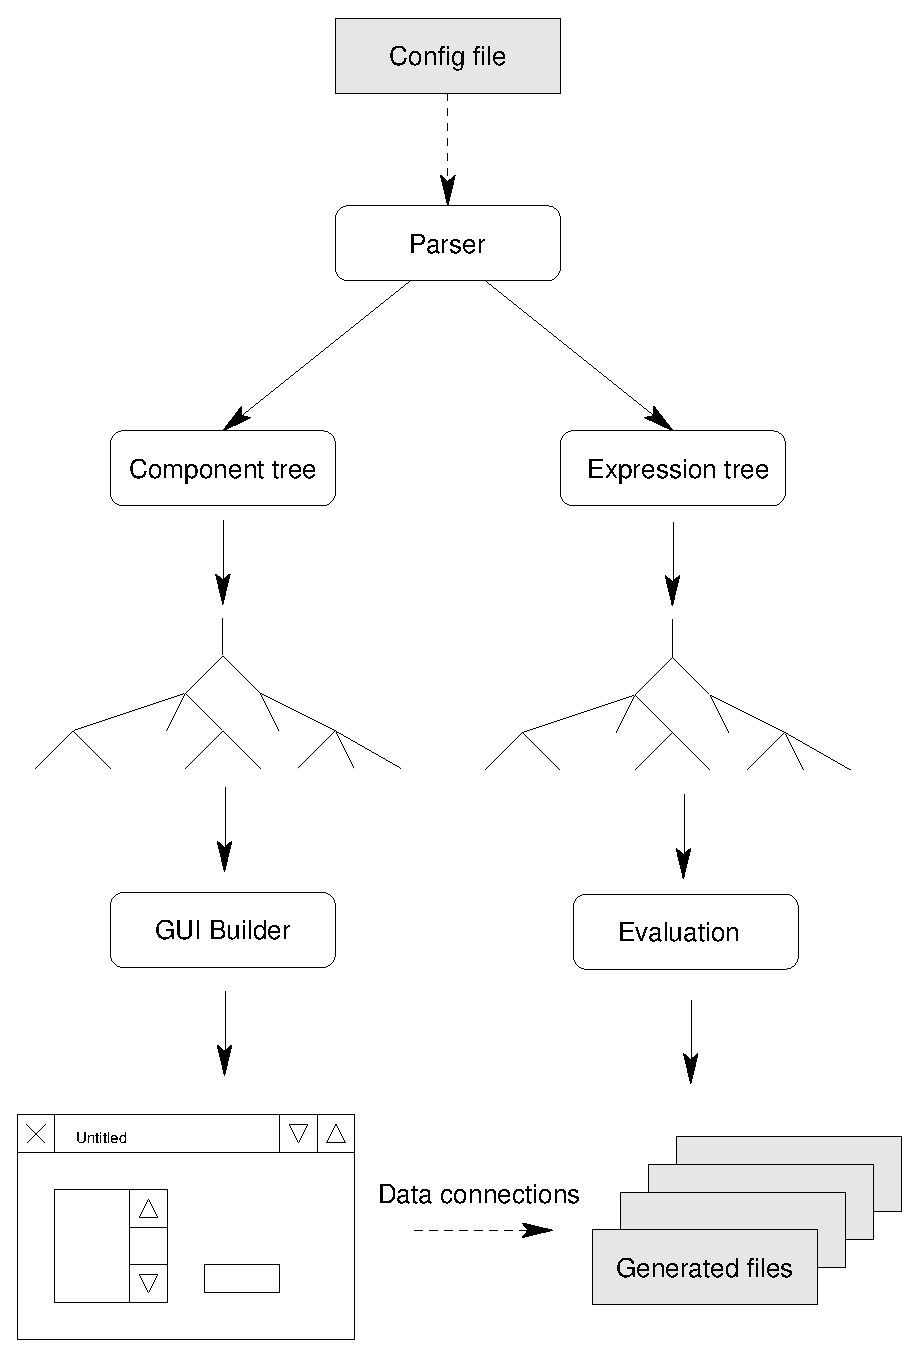
\includegraphics[width=9cm]{./figures/app_overview_new.eps}
    \caption{General view of how the application performs its task}
    \label{fig:design:overview}
\end{center} \end{figure}
The main function of the application --- generating files based on some
configuration and the users input --- is quite clear in this picture. The
entire process can be summarized as follows:
\begin{itemize}
\item Read and parse the configuration file containing a user interface
description and technology file format specifications.
\item Build the the technology file generators and build the user
interface using a ``component tree''.
\item Use the generators and the data entered in the user interface to generate
the required files.
\end{itemize}
First, the configuration file is read. The configuration file contains a
description of the user interface as well as information on how to generate the
required technology files. The user interface description actually specifies
\emph{what} data the user must enter and also \emph{how} the user must do this.
The technology file generator specification contains literal pieces of files as
well as references to elements in the user interface that will be substituted
with entered values. For more information on the format of this file see
\mbox{Chapter \ref{chap:language}}.

To efficiently build the user interface, a component tree is first created.
This component tree is then used to build the actual Qt
widgets\footnote{Widgets are the basic elements a user interface consists of,
e.g. buttons, listboxes, checkboxes, etc.}. A precise description of this
process can be found in \mbox{section \ref{sect:design:uibuilder}}.

The last step is file generation. To be able to generate the technology files,
data is collected from the user interface and fed into the file generators,
resulting in the required files.

%%%%%%%%%%%%%%%%%%%%%%%%%%%%%%%%%%%%%%%%%%%%%%%%%%%%%%%%%%%%%%%%%%%%%%%%%%%%%
\section{User interface architecture} \label{sect:design:ui_architecture}
The user interface can be separated into two parts. The first part handles
opening and closing files and file generation requests. It also provides an
interface for the second part. This first part will be called the
``framework''.

The second part of the user interface is the part of the user interface that is
described in the configuration file. This part specifies what data must be
entered (and how) to be able to generate a certain file. This second part will
be called the generated user interface.

%Since this is open to change we cannot be as specific as for the framework.

\subsection{The framework}
The framework used is just an implementation of the well-known multiple
document interface (MDI). The framework provides the actions the user expects
to find in a multiple document interface:
\begin{itemize}
\item Creating a new file
\item Opening (loading) of a file
\item Saving of a file
\item Closing of a file
\item Switching between open files
\end{itemize}
If we translate this abstraction to our case, the ``file'' is a process
description. Switching between files means that the user would like to start
editing on another process. The actions provided are grouped together in the
``File'' menu, as is common practice. The interested reader is referred to an
excellent book on user interface standards by Fowler and Stanwick
\cite{Fowler}.

\begin{table}[b] \begin{center}
\caption{Partial list of methods provided by the CProcessManager class.}
\label{tab:design:CProcessManager}
\begin{tabular}{l|p{6cm}}
\hline
 \textsf{Method}   & \textsf{Description}                                               \\
\hline
 \verb=currentProcess()=  & Gives a pointer to the process currently being edited by the user. \\
 \verb=newProcess()=      & Creates a new process and makes it the current process.            \\
 \verb=activateProcess()= & Switches to a new process.                                         \\
 \verb=removeProcess()=   & Closes and removes the process from the process manager.           \\
 \verb=saveProcess()=     & Saves a process to disk.                                           \\
 \verb=loadProcess()=     & Loads a process from disk.                                         \\
 \verb=generateFile()=    & Generates the requested technology file for this process.          \\
\hline
\end{tabular}
\end{center} \end{table}

In the implementation, the multiple document interface can mainly be found in
three classes: \verb=CAppMainWindow=, \verb=CProcessManager= and
\verb=CProcess=. The \linebreak \verb=CAppMainWindow= class receives the
signals given by the user whenever he selects one of the actions mentioned
before. The \verb=CProcessManager= class methods are then called to perform the
actions. This usually involves an operation on a \verb=CProcess= class
instance. All instances of the \verb=CProcess= class are ``registered'' and
managed by the \verb=CProcessManager= class. The most important methods
provided by the \verb=CProcessManager= class are listed in Table
\ref{tab:design:CProcessManager}. The \verb=CProcess= class will be discussed
again in Section \ref{sect:design:filegeneration}, since it is also part of the
file generation process.


\subsection{The generated user interface} \label{sect:design:generatedui}
\suppressfloats[t] The part of the user interface that is specified in the
configuration file is open to change. However, we must specify how this part of
the user interface integrates with the framework.

The most straightforward approach is to put all the user interface elements
specified inside the client area (the application window minus the menus,
toolbar and status bar). However, this is not a very practical approach. The
amount of data that must be entered and thus the number of input fields in the
user interface is large. This results in a too big and thus obscure scrollable
area.

\bigskip \noindent
A solution is to make it possible to ``partition'' the user interface. Each of
these parts can correspond to a file, or a certain aspect of the process
description. For example, a part can contain all information about the layers
in a process.

\begin{figure}[h!] \begin{center}
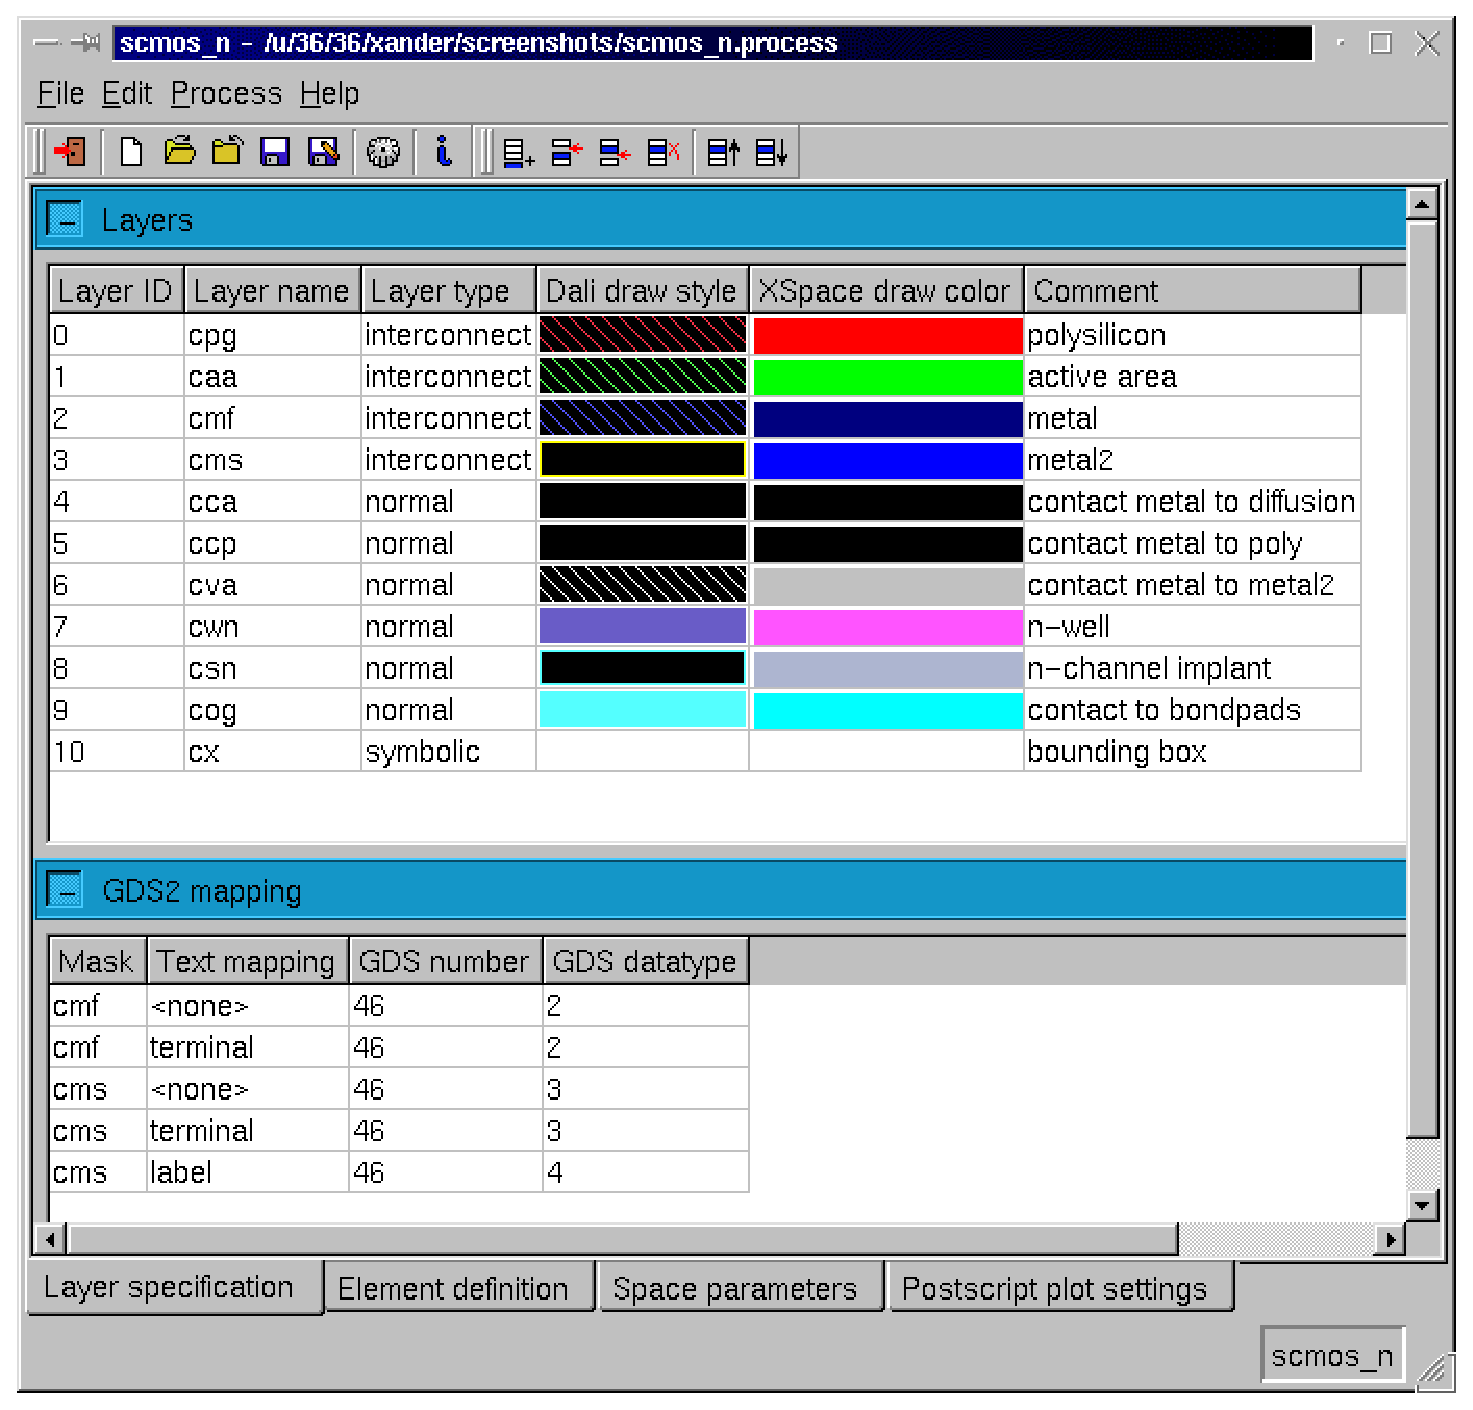
\includegraphics[width=7cm]{./figures/partition.eps}%mainwindow_layers.eps}
\caption{Partitioning and subpartitioning. The tabpages represent the first
level of partitioning. The sections (the blue horizontal bars) provide the
subpartitioning.}
\label{fig:design:tabpages}
\end{center} \end{figure}


These ``parts'' can still contain much data that must be entered. The element
definition file is good example of this. It would be better if we partition
each part even further. An effective user interface must thus be able to handle
partitions with sub-partitions.

\bigskip \noindent
The big question is now how we can achieve this. The first rough partitioning
that corresponds to the files can be implemented using ``tabpages''. Each
tabpage will correspond to a file or a general aspect of the process
description. The elements on the tabpage will describe the data that must be
entered.

As mentioned before, it would be profitable if we could further partition a
tabpage. Some files just will not fit on a tabpage. For this purpose, a custom
widget named the ``section'' widget was designed. It is described in detail in
Section \ref{sect:uidesign:section}. With this widget, a tabpage can be divided
into multiple sections, that can be shown either expanded or collapsed. A
collapsed section hides a part of its interface. This mechanism allows for a
much clearer arrangement of the user interface. Figure
\ref{fig:design:tabpages} shows the tabpages and sections in action.


%%%%%%%%%%%%%%%%%%%%%%%%%%%%%%%%%%%%%%%%%%%%%%%%%%%%%%%%%%%%%%%%%%%%%%%%%%%%%
\section{Design methodology and conventions}
Before each part of the design is discussed some remarks about the design
methodology and the used conventions are is place.

\bigskip \noindent
The \emph{Design Patterns} as described by Erich Gamma et al \cite{Gamma} are
used in the discussion of several parts of the design. These design patterns
provide a common vocabulary for computer program designers and therefore
references to these patterns will occur throughout the text.

\bigskip \noindent
Doxygen was used to generate the source code documentation. It is also capable
of generating so-called collaboration graphs, although the term collaboration
graph can be a bit misleading. The collaboration graphs generated by
\verb=doxygen= are a mix of what are called class diagrams and collaboration
diagrams in some well-known notations like Booch or UML.

In several places the collaboration graphs generated by
\verb=doxygen=\cite{doxygen} are used. Doxygen is a source code documentation
generator. The term

%%%%%%%%%%%%%%%%%%%%%%%%%%%%%%%%%%%%%%%%%%%%%%%%%%%%%%%%%%%%%%%%%%%%%%%%%%%%%
\section{The parser} \label{sect:design:parser}
To be able to read and interpret the configuration file, a parser has been
created. The parser consists of three parts (as shown in Figure
\ref{fig:design:parser}):
\begin{enumerate}
\item a lexical analyzer
\item a grammar parser
\item a class that provides methods for the parser to build the component tree
and the generators.
\end{enumerate}
The lexical analyzer scans the configuration file for keywords and other
special language elements like string delimiters and parentheses. The lexical
analyzer used is generated by \emph{flex}\footnote{flex is a lexical analyzer
based on and compatible with lex.}. Recognized keywords and elements are called
\emph{tokens}.

The lexical analyzer is used by the grammar parser. This grammar parser can
recognize and analyze a series of \emph{tokens}. It can then perform actions
related to the sequence of tokens it encountered. The grammar parser is
generated with \emph{bison}\footnote{bison is a parser based on and compatible
with the well-known grammar parser yacc.}. For more information about the
language used in the configuration file, please refer to \mbox{Chapter
\ref{chap:language}}.

\begin{figure} \begin{center}
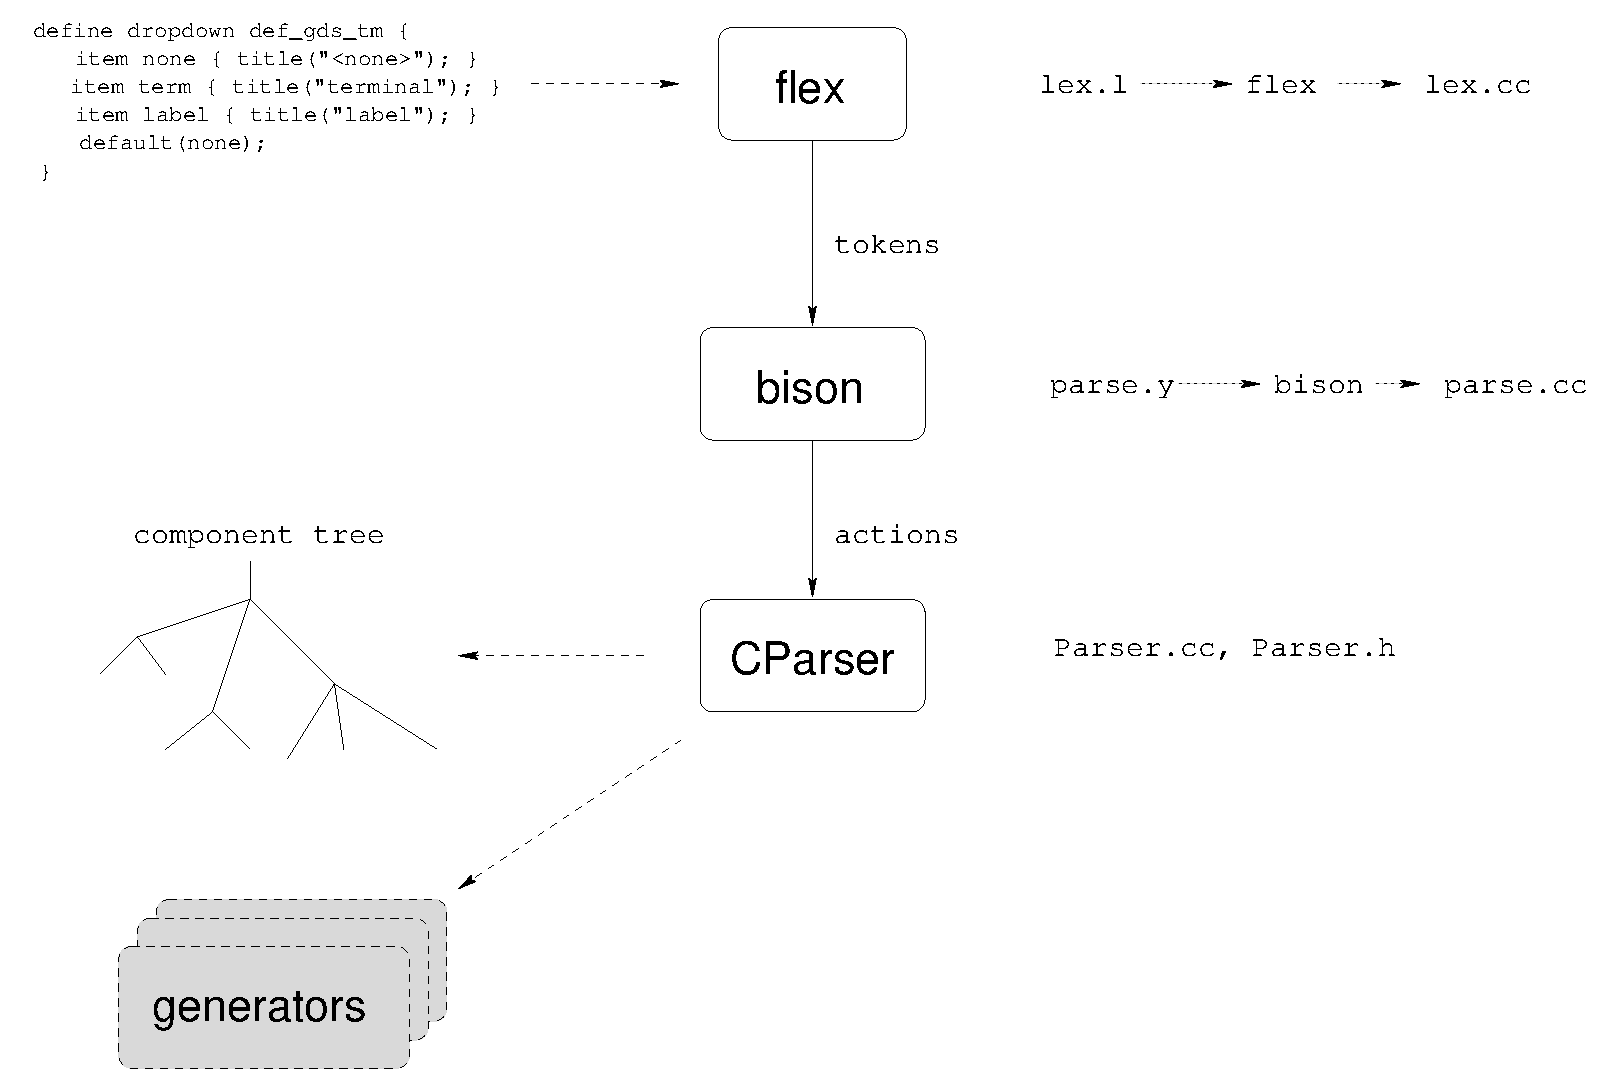
\includegraphics[width=12cm]{./figures/parser.eps}
\caption{The path from configuration file to component tree and generator data
structures. On the right side the files containing the implementation.}
\label{fig:design:parser}
\end{center} \end{figure}

The actions that the parser performs are the methods provided by the parser
class, \verb=CParser=. The \verb=CParser= class builds the component tree and
the generators, which are described in the following sections. The
\verb=CParser= class also extends the functionality of the parser generated by
bison:
\begin{itemize}
\item Disambiguation of identifiers specified in the configuration file. If
ambiguities arise, these are reported. \item The \verb=CParser= class also acts
as a \emph{builder}\footnote{A simplified version of the \emph{builder} pattern
described by Gamma et al \cite{Gamma} is used here.} for the component trees
and generators.
\item The \verb=CParser= class is implemented as a \emph{singleton}\footnote{The
\emph{singleton} pattern as described by Gamma et al \cite{Gamma}.}. This
ensures that only one instance of the parser will be created and that this
instance will be easily accessible.
\item Errors in the configuration file are reported in a dialog box in
stead of on the console. The line number of the line(s) containing the error(s)
are also reported.
\end{itemize}

%%%%%%%%%%%%%%%%%%%%%%%%%%%%%%%%%%%%%%%%%%%%%%%%%%%%%%%%%%%%%%%%%%%%%%%%%%%%%
\section{Components and the component tree} \label{sect:design:components}
The parser described in the previous section creates a tree, as is illustrated
in Figure \ref{fig:design:overview} and Figure \ref{fig:design:parser}. This
tree is called the component tree and consist of instances of the
\verb=CComponent= class.

In the following sections, the structure and abilities of the component tree
will be explained.

\subsection{Structure}
The tree is based on the \emph{composite} pattern, as described in Gamma et al
\cite{Gamma}. The difference between the composite pattern and the structure
used here is the lack of the ``leaf'' nodes. Only the ``composite'' nodes are
used in the component tree. The reasons for this are simple:
\begin{itemize}
\item The number of nodes in the component tree is relatively small. The
argument of efficient memory usage by using separate classes for leaves and
composite nodes is a weak one in this case.
\item The complexity decreases, thereby simplifying implementation.
\end{itemize}
Root components are tied together in the \verb=CComponentTree= class. The
collaboration graph for the \verb=CComponentTree= is shown in \mbox{Figure
\ref{fig:doxygen:CComponentTree_coll}}

\begin{figure}[ht]
\begin{center}
\includegraphics[height=2cm]{./figures/class_ccomponenttree_coll_graph.eps}
\caption{CComponentTree collaboration graph.}
\label{fig:doxygen:CComponentTree_coll}
\end{center}
\end{figure}
As can been seen in \mbox{Figure \ref{fig:doxygen:CComponentTree_coll}} the
\verb=CComponentTree= contains references to the \verb=CComponents= that are
root components. The \verb=CComponent= class contains references to
\verb=CComponents= that are either the parent component (\verb=m_parent=) or
child components (\verb=m_children=).

\subsection{CComponent and CComponentTree abilities}
\label{sect:design:component_abilities}
The \verb=CComponent= class provides the following functionality for its
clients:
\begin{itemize}
\item Name and context methods
\item Property support
\item Simple type support
\item Parent/child access
\end{itemize}

\bigskip \noindent
\textbf{Name and context methods} control access to the components name.
Components have names that function as an identifier. The names of the parent
components concatenated with dots form the ``context'' in which the identifier
lives. For example, if \verb=A= is a parent of \verb=B= and \verb=B= is the
parent of
\verb=C= then \verb=A.B= is the context of \verb=C= and \verb=A.B.C= is the
``full-context name'' of component \verb=C=.

Access to names and contexts is provided by the \verb=setName()=,
\verb=getName()= and \verb=getFullContextName()= methods.

\bigskip \noindent
\textbf{Property support} is something not provided by C++. C++ requires
explicit set and get methods for class members. Properties would be very useful
for the
\verb=CComponent= class. Many different types of components will be described
by the \verb=CComponent= class and properties would make this easier.
Inheritance is also an option, but the number of classes required would be too
large to implement in the given time.

Property support is therefore added to the \verb=CComponent= class by providing
methods like \verb=setProperty()= and \verb=getProperty()=. The properties are
stored in the STL\footnote{STL is the Standard Template Library, which is part
of the C++ standard. The STL provides containers, algorithms, strings, streams
and many other utility classes.} container \emph{map}. A property can have
\emph{multiple} values, because the values are stored as a vector of strings.
For more implementation specifics, please refer to the source code
documentation \cite{SPOCK}.

\bigskip \noindent
\textbf{Simple type support} must be present to be able to differentiate
between the component types. Type support is very crude, only methods like
\verb=setType()= and \verb=getType()= are implemented. There is currently no
support for type checking and type conversion.

\bigskip \noindent
\textbf{Parent/child access} and modification is also provided. The available
methods include:
\begin{itemize}
\item \verb=getParent()= retrieves a pointer to the parent component
\item \verb=add()= adds a child to this component
\item \verb=removeChild()= removes a child from the list of children
\item \verb=getChild()= can retrieve a pointer to a child component
\item \verb=numChildren()= and \verb=childPos()= provide array--like access to
the children.
\end{itemize}
Some of these methods have multiple implementations accepting different
arguments, increasing the flexibility of this much--used class.

\subsection{Component tree creation}
A prototype tree is created by the \verb=CParser= class described in
\mbox{Section \ref{sect:design:parser}}. The prototype tree is copied for every
process that is created with ``File $\rightarrow$ new'' or loaded into the
application. The reasons for this will be explained further in \mbox{Section
\ref{sect:design:uibuilder}}, where the user interface builder is described.

\subsection{Iterating through the component tree}
Iterating through the tree is necessary for building the user interface,
searching components, printing debug information about the components, etc.
Walking through the tree is such a common action that the interface should be
open to extension.

The \emph{visitor} pattern is applied to make the interface flexible. The
visitor pattern allows us to easily apply an operation to the component tree.
Some of the advantages of using the visitor pattern:
\begin{itemize}
\item The \verb=CComponent= class is not polluted by methods and attributes related to
a certain operation on the entire tree. This related behaviour is placed in the
visitor class instead.
\item The visitor pattern makes it easy to define new operations on the tree.
Adding a new visitor is all that is required.
\item Visitors can also accumulate state as they visit each component in the
component tree. This is done for example in the FindComponentVisitor, which
counts the number of hits.
\end{itemize}
The visitor pattern is described in Gamma et al. \cite{Gamma}.

\subsubsection*{Available visitors}
The available and by \verb=CComponentTree= accepted visitors are listed in
Table \ref{tab:design:visitors}. The implementation of the
\verb=CFindComponentVisitor=, \verb=CFindPropertyVisitor= and
\verb=CDumpComponentTreeVisitor= is straightforward and the interested reader
is referred to the source code documentation.
\begin{table}
\caption{Visitors and their purpose}
\label{tab:design:visitors}
\begin{tabular}{l|p{6cm}}
\hline
 \textsf{Visitor} & \textsf{Description} \\
\hline  %\hline
    \verb=CFindComponentVisitor= & Retrieves all components with a given name. \\
%\hline
    \verb=CFindPropertyVisitor=  & Retrieves all components that have the specified
    property. The value specified is compared with the value of the property
    considered. The comparison criterion can be specified as either equal or
    unequal. This could be extended with larger/smaller criteria in future
    versions. \\
%\hline
    \verb=CDumpComponentTreeVisitor= & This visitor prints the (indented)
    tree to the console. This visitor is provided for debugging purposes. \\
%\hline
    \verb=CGUIBuilderVisitor= & The GUI build process is described in detail in
    \mbox{Section \ref{sect:design:uibuilder}}.\\
    \verb=CSerializerVisitor= & Provides means to load or save the information
    entered by the user and stored in this tree. This is discussed in Section \ref{sect:design:serialization}\\
\hline
\end{tabular}
\end{table}

\verb=CSerializerVisitor= and \verb=CGUIBuilderVisitor= are not so
straightforward. The \verb=CGUIBuilderVisitor= class is described in detail in
Section \ref{sect:design:uibuilder}. The \linebreak \verb=CSerializerVisitor=
and serialization\footnote{Serialization is the term used for the process of
saving and loading application data.} in general is discussed in Section
\ref{sect:design:serialization}.


%%%%%%%%%%%%%%%%%%%%%%%%%%%%%%%%%%%%%%%%%%%%%%%%%%%%%%%%%%%%%%%%%%%%%%%%%%%%%
\section{The user interface builder}\label{sect:design:uibuilder}
So, after parsing the configuration file the component tree is created and
ready to be processed further. The user interface builder creates the actual
widgets (the basic user interface elements) from the component tree by visiting
the tree with the \verb=CGUIBuilderVisitor=.

The creation of the user interface is thus a two step process:
\begin{enumerate}
\item The component tree with the structure of the user interface is created
from the configuration file.
\item The \verb=CGUIBuilderVisitor= visits the component tree and creates a
\verb=CGUITree= object that contains the created widgets and provides methods
to access them.
\end{enumerate}

One might wonder why the component tree does not contain the widgets and why
the \verb=CGUIBuilderVisitor= is needed. After all, all the information related
to the user interface is already ``in there''. The reasons behind this are
actually quite straightforward:

\begin{itemize}
\item The hierarchy Qt uses for its widgets is different from the one used by
the component tree. The Qt tree is very fine-grained compared with the
component tree and incorporates layout information for the widgets.
\item If we were to include the creation and management of the Qt widgets in
the component tree, the \verb=CComponent= class would get ``bloated''. The
\verb=CComponent= class would serve two different purposes (\verb=CComponent=
parent/child management and Qt widget management), which is usually bad
software engineering.
\end{itemize}

\subsection{The CGUIBuilderVisitor}
The \verb=CGUIBuilderVisitor= first determines the type of the component being
visited. It then calls the method needed to build that type of component. These
(private) methods are listed in Table \ref{tab:design:CGUIBuilderVisitor}.

The widgets created are mapped to the components whenever this is desired. This
mapping allows us to access the value a user enters in the widget using the
\verb=CGUITree=. The mapping is described in detail in the next section.

\begin{table} \begin{center}
\caption{CGUIBuilderVisitor build methods.}
\label{tab:design:CGUIBuilderVisitor}
\begin{tabular}{l|p{6cm}}
\hline
 \textsf{Method}          & \textsf{Description}                                                                                                                     \\
\hline
 \verb=buildTabPage()=           & Creates a tabpage. A tabpage usually contains only a scrollframe.                                                                 \\
 \verb=buildScrollFrame()=       & Creates a scrollframe. A scrollframe can contain multiple widgets. If they do not fit inside the frame, scrollbars are displayed. \\
 \verb=buildSection()=           & Creates a section. A section can contain multiple widgets, including nested sections.                                             \\
 \verb=buildParamList()=         & Creates an empty parameter list.                                                                                                  \\
 \verb=buildSpreadSheet()=       & Creates an empty spreadsheet.                                                                                                     \\
 \verb=buildSpreadSheetColumn()= & Adds a column to the current spreadsheet.                                                                                         \\
 \verb=buildComboBox()=          & Creates combobox and dropdown widgets.                                                                                            \\
 \verb=buildLineEdit()=          & Creates a line edit.                                                                                                              \\
\hline
\end{tabular} \end{center} \end{table}


\subsection{The CGUITree}
The \verb=CGUITree= created by the \verb=CGUIBuilderVisitor= provides a mapping
between a component tree and the Qt widgets related to that tree. The methods
provided reflect this.

\paragraph{The mapping methods} allow creating a mapping and retrieval of
values from the mapping. To create a mapping between a component and a widget
\verb=makeMapping()= can be used. To retrieve either a component given a widget
or a widget given a component, \verb=getComponent()= or \verb=getWidget()= can
be used. As a special case, \verb=getTabPages()= retrieves all the tabpages in
the gui tree.

\paragraph{Value methods} are also implemented. These consist of get/set
methods for normal components and get/set methods for spreadsheets. The
spreadsheet methods take the column component as an extra argument. The methods
are named \verb=getValues()=, \verb=setValues()=, \verb=getSpreadSheetValues()=
and \linebreak \verb=setSpreadSheetValues()=.

\paragraph{Other methods} provided include methods for data connections, which
will be discussed in Section \ref{sect:design:dataconnections}.
\verb=findComponent()= is implemented as a convenience function. It calls the
associated component tree's \verb=findComponent()= method. Also implemented are
some slot\footnote{slots are part of Qt's signal/slot mechanism which allow
sending and receiving signals to and from objects.} methods needed by the
spreadsheets. More about this in Section \ref{sect:uidesign:spreadsheet} where
the spreadsheet widget is explained.

\bigskip \noindent
A partial collaboration diagram showing the classes discussed is presented in
Figure \ref{fig:design:guibuilder_partial}.

\begin{figure} \begin{center}
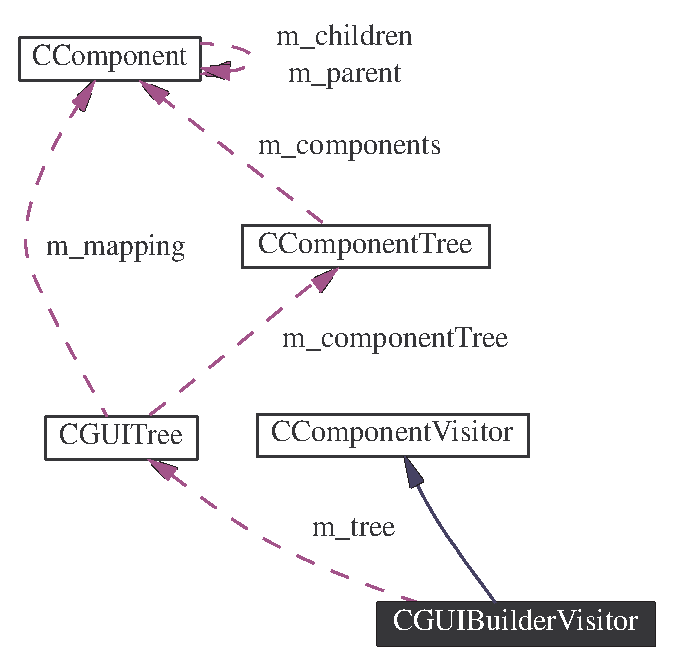
\includegraphics[width=7cm]{./figures/guibuilder_partial.eps}
\caption{Partial collaboration diagram for class CGUIBuilderVisitor}
\label{fig:design:guibuilder_partial}
\end{center} \end{figure}

%%%%%%%%%%%%%%%%%%%%%%%%%%%%%%%%%%%%%%%%%%%%%%%%%%%%%%%%%%%%%%%%%%%%%%%%%%%%%
\section{Data connections} \label{sect:design:dataconnections}
An important feature that partly determines the success of the chosen approach
is the ability to use the data entered by the user in other fields. For
example, in some part of the user interface the user must specify which layers
exist in the application. In some other part, the user must map a layer to a
GDS2 number. It would be convenient if the user could choose from the defined
layers. This not only reduces the chance of (typing) errors, it also makes the
user interface more comfortable to work with.

\bigskip \noindent
This dynamic behaviour is implemented by the data connection classes. A data
connection consists of one or more data sources, a single data target and a
data connection object that is responsible for the actual synchronization of
values between the sources and the target. This is depicted in Figure
\ref{fig:design:dataconnections}.

\begin{figure} \begin{center}
\includegraphics[width=12cm]{./figures/class_cdataconnection_coll_graph.eps}
\caption{Data connection collaboration diagram.}
\label{fig:design:dataconnections}
\end{center} \end{figure}

The implementation relies heavily upon the Qt signal/slot mechanism. This
mechanism implements the \emph{observer} pattern \cite{Gamma}. The dynamics of
this construction are expressed in Figure \ref{fig:design:datadynamics}. The
\verb=CDataSource= object ``detects'' a change in the value it watches. It then
signals the \verb=CDataConnection= object that the target needs updating. The
\verb=onSynchronize()= method then calls \verb=updateValues()= for the correct
\verb=CDataTarget= object.

%% figure goes here.
\begin{figure} \begin{center}
\includegraphics[width=10cm]{./figures/dataconnection_dynamics.eps}
\caption{Example of Qt's signal/slot mechanism.}
\label{fig:design:datadynamics}
\end{center} \end{figure}

Currently, there is only one type of data source supported. This is the column
of a (custom) spreadsheet widget. The constructor checks if the source
component specified is a column in a spreadsheet. The \verb=getValues()= member
is tailored to retrieve the values from a spreadsheet column.

Support for different types of data sources can easily be added. The methods
involved are declared virtual. This means a new \verb=CDataSource= derived
class supporting the new type of source can easily be added.

The \verb=CDataTarget= class already has some derived classes. They are listed
(and explained) in Table \ref{tab:design:datatargets}.

\begin{table} \begin{center}
\caption{Possible data targets.}
\label{tab:design:datatargets}
\begin{tabular}{l|l}
\hline
 \textsf{Derived class name}     & \textsf{Description}                          \\
\hline
 \verb=CColumnDataTarget=        & The data target is a column in a spreadsheet. \\
 \verb=CComboDataTarget=         & The data target is a combobox like component  \\
 \verb=CConditionListDataTarget= & The data target is a condition list.          \\
\hline
\end{tabular}
\end{center} \end{table}

%%%%%%%%%%%%%%%%%%%%%%%%%%%%%%%%%%%%%%%%%%%%%%%%%%%%%%%%%%%%%%%%%%%%%%%%%%%%%
\section{Technology file generation} \label{sect:design:filegeneration}
The file generation architecture strongly resembles the architecture used to
build the user interface. Figure \ref{fig:design:filegeneration} presents this
architecture. If we compare this process with the one that creates a user
interface we can see a lot of similarities. Both start from a definition given
in the configuration file. This definition is then parsed and a component tree
is created.

\begin{figure} \begin{center}
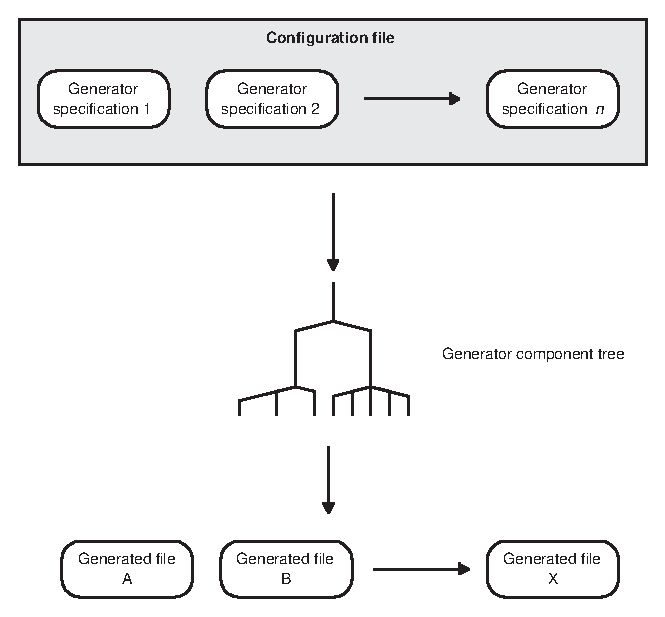
\includegraphics[width=8cm]{./figures/file_generation.eps}
\caption{Overview of the file generation process.}
\label{fig:design:filegeneration}
\end{center} \end{figure}

The datastructures used for the file generation process are discussed next,
followed by a description of the generation process itself.

\subsection{File generation datastructures}
As mentioned before, the format specifications defined in the configuration
file are parsed and put into an expression tree. Like the component tree, this
tree structure uses the \verb=CComponent= class for its nodes. However, the
tree interpretation is different. The nodes of the component tree represent a
part of a hierarchy, while the nodes of the expression tree represent an action
that should be performed (possibly involving the nodes' children).

For the file generator, the nodes in the tree can all be evaluated to plain
text. The tree structure represents the more elaborate language constructs,
like the \verb=foreach= loops and \verb=if= constructions. These constructs can
affect the eventual result. More information on these language constructions
can be found in Chapter \ref{chap:language}.

\bigskip \noindent
The root components of the tree represent the generators. The class used for
the root components is the \verb=CGeneratorComp= component. This is a
\verb=CComponent= derived class. The added functionality lies in the support of
value maps.

A value map allows the ``translation'' of dropdown item text to the text that
should be generated instead. This mapping applies to all instances of the
dropdown in that tree. In a future version of the application this behaviour
could be extended to include other types of substitution as well.

\bigskip \noindent
The generators are collected in the \verb=CGenerators= class. Currently, the
interface only provides methods for access to the generators. They are listed
in Table \ref{tab:design:CGenerators}.

\begin{table} \begin{center}
\caption{Methods provided by the CGenerators class}
\label{tab:design:CGenerators}
\begin{tabular}{l|l}
\hline
 \textsf{Method}          & \textsf{Description}  \\
\hline
 \verb=addGeneratorComp()=       & Adds a generator to the list of generators.\\
 \verb=numGenerators()=          & Returns the number of generators. \\
 \verb=getGenerator()=           & Retrieves the desired generator.\\
\hline
\end{tabular} \end{center} \end{table}

The \verb=CGenerators= class could be extended with additional methods if the
need for them arises.

\subsection{The generation process}
Generating the files starts with the user bringing up the generation dialog
box. As can be seen in Figure \ref{fig:design:generatedialog} each file can be
generated separately. The result can be saved into a specified directory or
into the SPACE process tree directly (if the user has the required rights).
This is explained in detail in Section \ref{sect:design:integration}. Before
the files are actually written to disk they can be inspected and edited if the
user checks the ``Edit and inspect results'' option.

\begin{figure}[!bh] \begin{center}
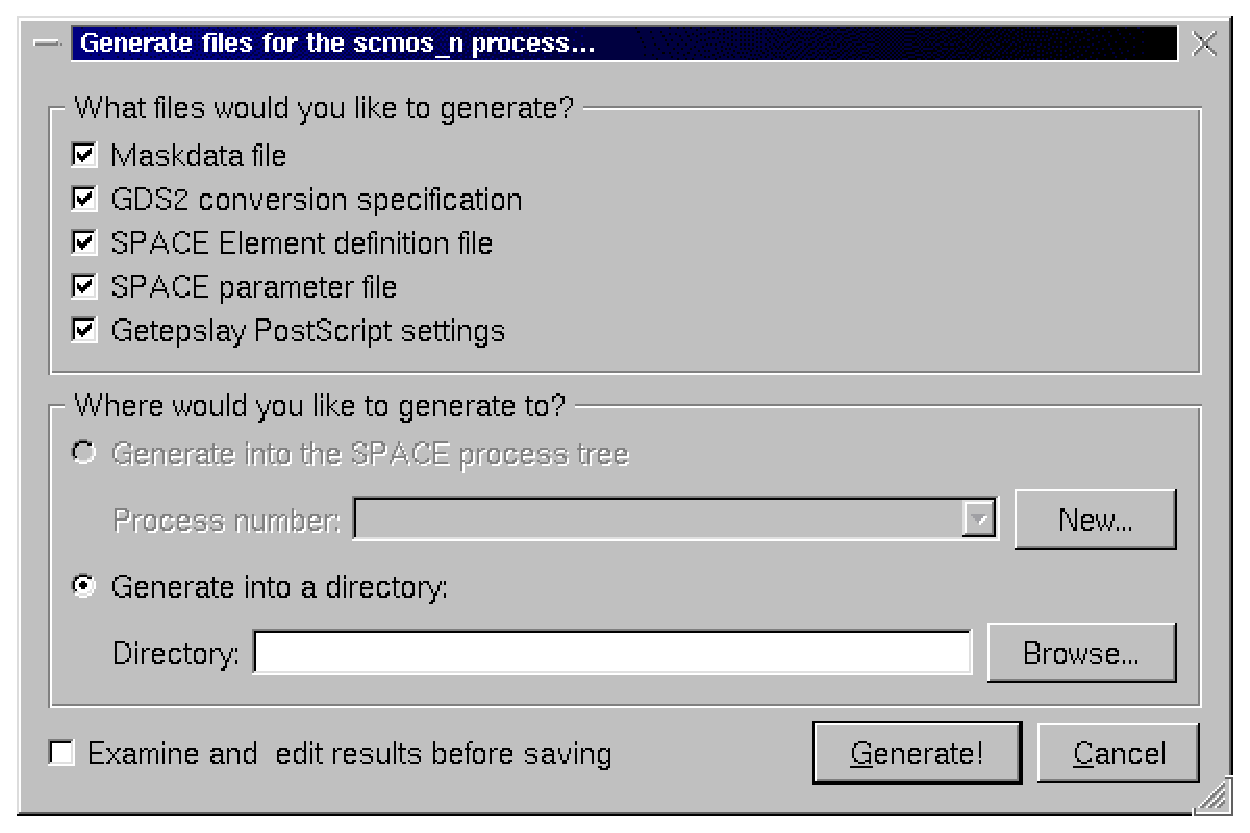
\includegraphics[width=7cm]{./figures/generate.eps}
\caption{The technology file generation dialog box.}
\label{fig:design:generatedialog}
\end{center} \end{figure}
After all the required information is gathered, the \verb=generateFile()=
method from the \verb=CProcess= class is called for each file that must be
generated. This method evaluates the file's generator tree to the file's
contents. The evaluation of the nodes is done by some private helper methods
included in the \verb=CProcess= class. They include the generation of literals,
identifiers, numbers, binary operators like addition and subtraction, \verb=if=
constructions and \verb=foreach= constructions. It is also possible to request
some information from the application. These include process name and
description and time and date of generation.

To allow nested \verb=foreach= loops a dedicated class was written that
contains the state of an iteration. The class is named \verb=CIteratedState=
and instances of this class are put into a stack by the \verb=CProcess= class
as necessary.

\subsection{Integration with the SPACE process tree} \label{sect:design:integration}
As was mentioned in the previous section, it is also possible to generate the
result directly into the SPACE process tree.

SPACE keeps the technology files for each process in a separate directory. The
name of the directory is also the name of the process. The process directories
all reside inside a directory that also contains the \verb=processlist= file.
This file contains a list of the processes mapped to a certain number. Changing
the number of a process is potentially dangerous and should be avoided.

To generate a process into the SPACE process tree, an update of the
\verb=processlist= file is required. The user must either select the correct
number or enter a new number for the process to be generated. To aid the user,
the comments after each mapping are read and displayed together with the
numbers and names of the processes in the \verb=processlist= file.

\bigskip \noindent
If the user proceeds with the generation process, the \verb=processlist= file
is rewritten to disk. The entry of the generated process is added or replaced
(depending on the users' choice for the process number). The comment after the
new entry will contain the process description.

%%%%%%%%%%%%%%%%%%%%%%%%%%%%%%%%%%%%%%%%%%%%%%%%%%%%%%%%%%%%%%%%%%%%%%%%%%%%%
\section{Serialization} \label{sect:design:serialization}
With serialization we mean storing or retrieving the data describing a process
to or from disk. The flexibility of the application makes this quite difficult
however, as will be explained in the following sections.

\subsection{Serialization method}
The data that must be serialized is entered by the user in the user interface.
The user interface is generated from the configuration file. This means that
the method used to serialize the data must somehow include this information.

The obvious solution is to bundle the data and the user interface description
present in the configuration file. However, this introduces a problem that is
unacceptable. The whole idea of the chosen approach was to introduce
flexibility. If we bundle the data and the user interface description, changes
made to the configuration file are useless. The old configuration file that was
bundled with the data will be used instead, thus effectively eliminating the
introduced flexibility.

\bigskip \noindent
To prevent the problem described above, the data is stored as key-value pairs.
The key is the full context name of the component associated with the data. The
value is the actual value in the user interface. This ensures that every value
can be restored, even if additions have been made to the configuration file.

Unfortunately, this approach has it defects as well. Defects that can largely
be overcome though.

\subsection{Compatibility issues}
The proposed method of serializing the data works as long as the full context
names of the components are still the same as in a newer configuration file.
Since the full context name also contains information about how the user
interface is arranged, moving parts of the user interface can be disastrous.

For example, in version 1 of the configuration file we have the component
\verb=A.B.C.D=. In version 2 we would like to have \verb=C.D= somewhere else.
Let us assume we want to move it to \verb=A.E=, resulting in \verb=A.E.C.D=. It
is clear that the old version 1 files cannot be read by the version 2
configuration file, although no real changes in the data have occurred.

To solve this problem, a disambiguation method has been implemented. If the
full context name cannot be resolved, context is added to the components name
until a single match is found. Continuing the previous example, this would mean
the search would start with \verb=D=. If \verb=D= is not unique, \verb=C= is
added to the context, resulting in \verb=C.D=. In this case, \verb=A.E.C.D= is
the unique component found.

\bigskip \noindent
Renaming components between versions is another issue. Renaming can be solved
by adding methods that can translate old version names to new version names.
This means editing source. As a result, renaming components is an action that
causes a major version change. This is acceptable, since renaming is mostly
done because of the esthetics of the configuration file.

Adding and removing components is no problem. Adding a component means the
component will be set to the default since it is not present in the old
version. Removing a component means that the component cannot be found if an
old version file is loaded. In this case, nothing happens.

\subsection{Implementation}
Because values are stored by their component name, a \emph{visitor} can be used
here. The visitor is called \verb=CSerializerVisitor=. The most important
methods are listed in Table \ref{tab:design:CSerializerVisitor}.

\begin{table} \begin{center}
\caption{Important methods provided by the CSerializerVisitor class}
\label{tab:design:CSerializerVisitor}
\begin{tabular}{l|p{6cm}}
\hline
 \textsf{Method}                  & \textsf{Description}                                                                                                  \\
\hline
 \textsf{readConversion()}        & While reading a file, converts an identifier-value pair from an old version to a new version. Currently does nothing. \\
 \textsf{writeConversion()}       & While writing a file, converts an identifier-value pair from this version to an old version. Currently does nothing.  \\
 \textsf{guessCorrectComponent()} & Tries to resolve relocated components.                                                                                \\
 \textsf{doFileInit()}            & Reads or writes the file header. The header contains the process name and description.                                \\
\hline
\end{tabular}
\end{center} \end{table}

\section{The application}
A screenshot of the application in action is shown in Figure
\ref{fig:design:app_screenshot}.

\begin{figure} \begin{center}
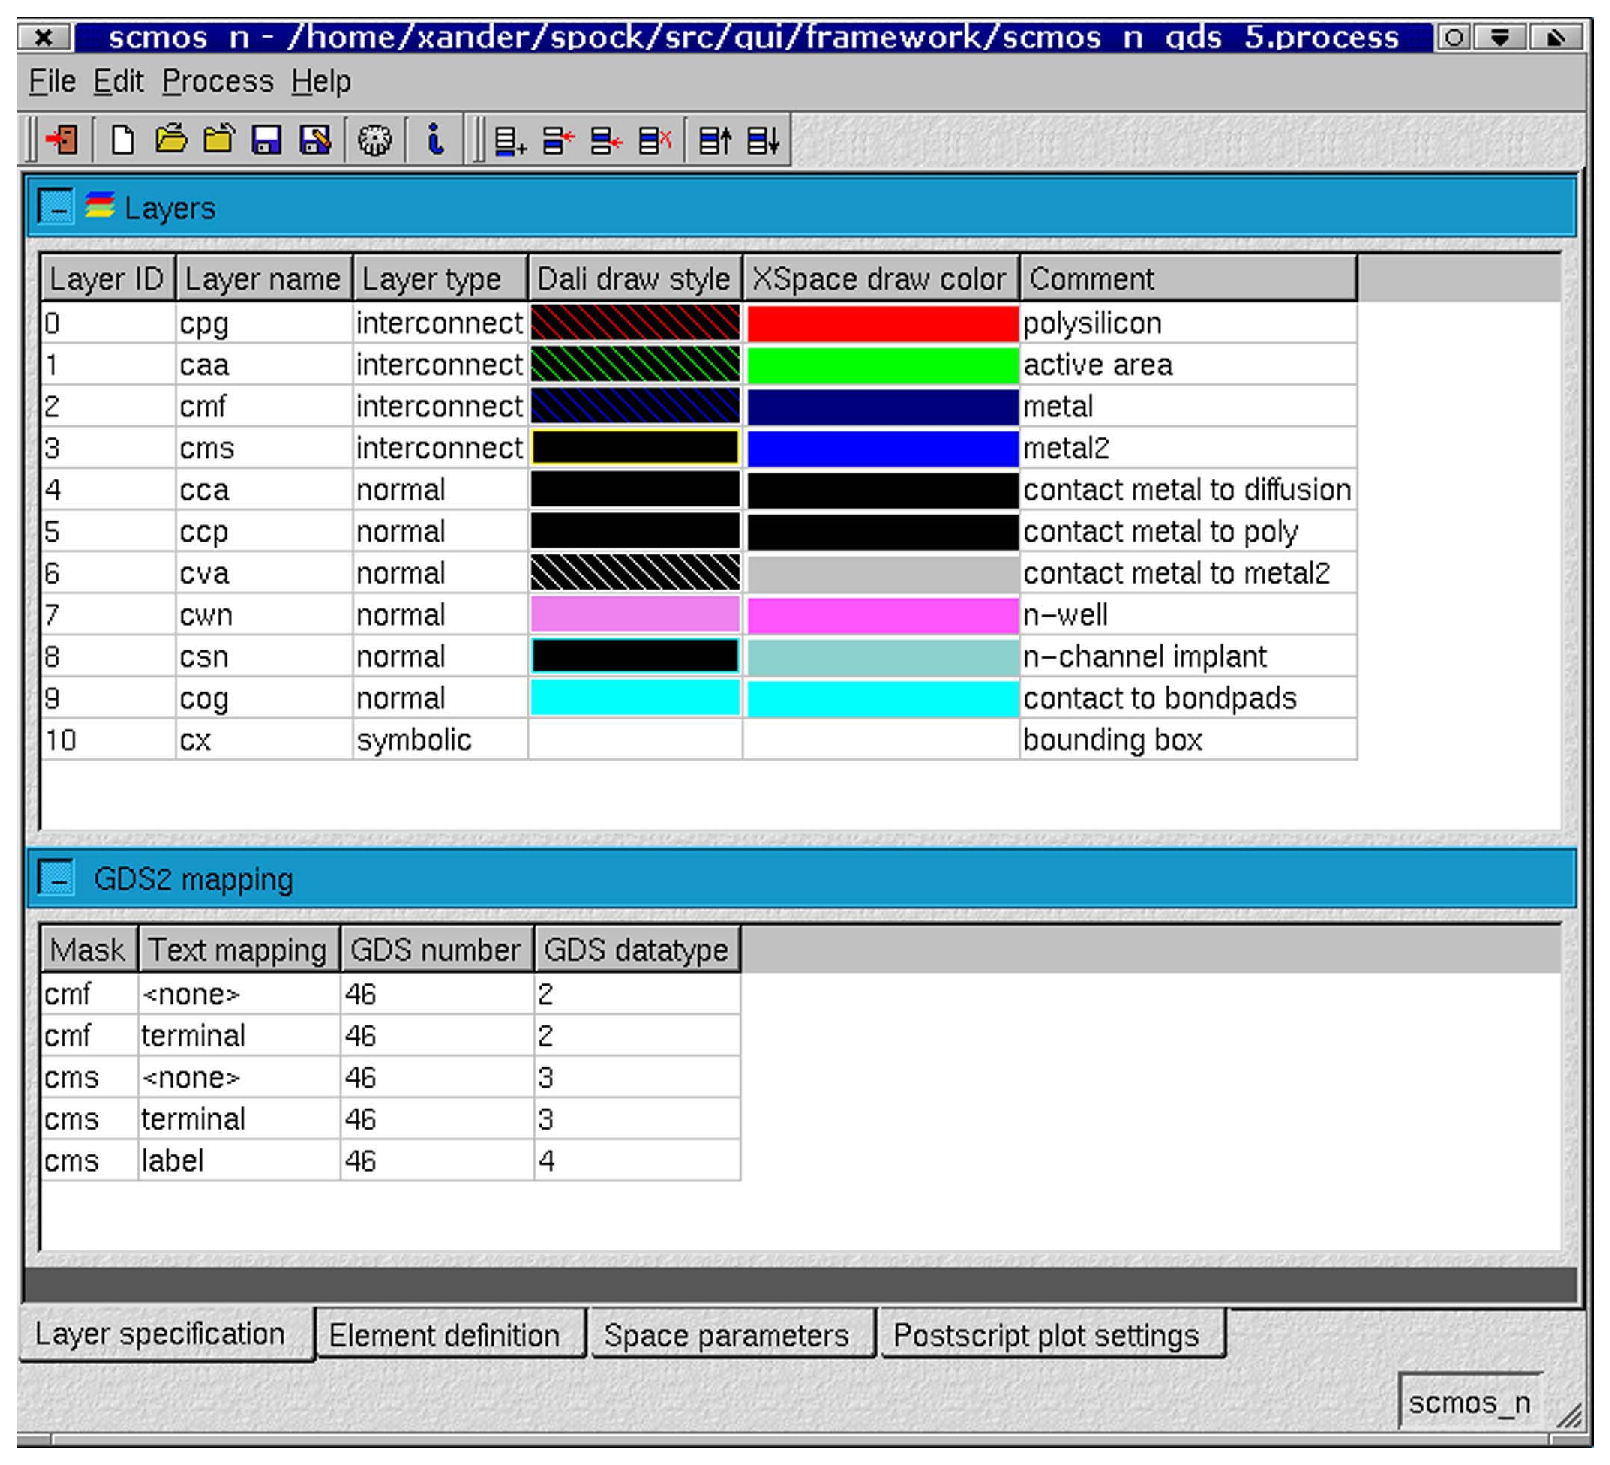
\includegraphics[width=8cm]{./figures/app_action.eps}
\caption{The application in action.}
\label{fig:design:app_screenshot}
\end{center} \end{figure}

As was already mentioned in Section \ref{sect:design:integration}, the
technology files can be generated directly into the SPACE process tree. This is
just one aspect of the relationship between the SPACE and the application.

\subsubsection*{Place of the configuration file}
The configuration file should be present either in the directory the
application was started from or in
\texttt{\$ICDPATH$\backslash$lib$\backslash$spock}. The filename should be
\verb=spock.uis=. If the file is not found in either location the application
will exit. \texttt{\$ICDPATH} is an environment variable that should point to
the SPACE installation location.

\subsubsection*{Existing technology files}
Unfortunately, existing technology files cannot be read by the application.
Only the processes entered in the application and saved in the applications'
own file format can be read.

%%%%%%%%%%%%%%%%%%%%%%%%%%%%%%%%%%%%%%%%%%%%%%%%%%%%%%%%%%%%%%%%%%%%%%%%%%%%%
\section{Recommendations for future features} \label{sect:design:future}
Although the application is already quite complete, there is always room for
improvement. Some recommendations were already mentioned somewhere in this
chapter. These recommendations are included in the list below.

\begin{itemize}
\item \textbf{Components and the component tree} \\ Better type support. Type
checking and type conversion routines could be implemented.
\item \textbf{Data connections} \\ Support for more types of data sources and
targets could be implemented.
\item \textbf{Generator value maps} \\ The value substitution method used by
the generators only supports substitution of dropdown and combobox values
defined in the configuration file. This mechanism could be extended to include
arbitrary substitution of values.
\item \textbf{Framework enhancements} \\ The framework user interface could be
extended to include cut, copy and paste operations. An undo/redo feature would
also be a useful addition.
\end{itemize}
\noindent Recommendations for the configuration file language can be found in
\mbox{Chapter \ref{chap:language}.}

%\begin{itemize}
%\item Components and the component tree
%    \begin{itemize}
%    \item Better type support. Type checking and type conversion routines
%    could be implemented.
%    \end{itemize}
%\item Data connections
%    \begin{itemize}
%    \item Support for more types of data sources and targets could be
%    implemented.
%    \end{itemize}
%
%\end{itemize}

%%%%%%%%%%%%%%%%%%%%%%%%%%%%%%%%%%%%%%%%%%%%%%%%%%%%%%%%%%%%%%%%%%%%%%%%%%%%%
\section{Graphical overview} \label{sect:design:conclusions}
In this last section a graphical overview of the completed and implemented
design is presented.

\bigskip \noindent
Figure \ref{fig:design:complete_overview} contains a complete high-level
overview of the design. Clearly visible are the similarities between the GUI
creation part of the application and the file generating part of the
application.

\begin{figure}[b!] \begin{center}
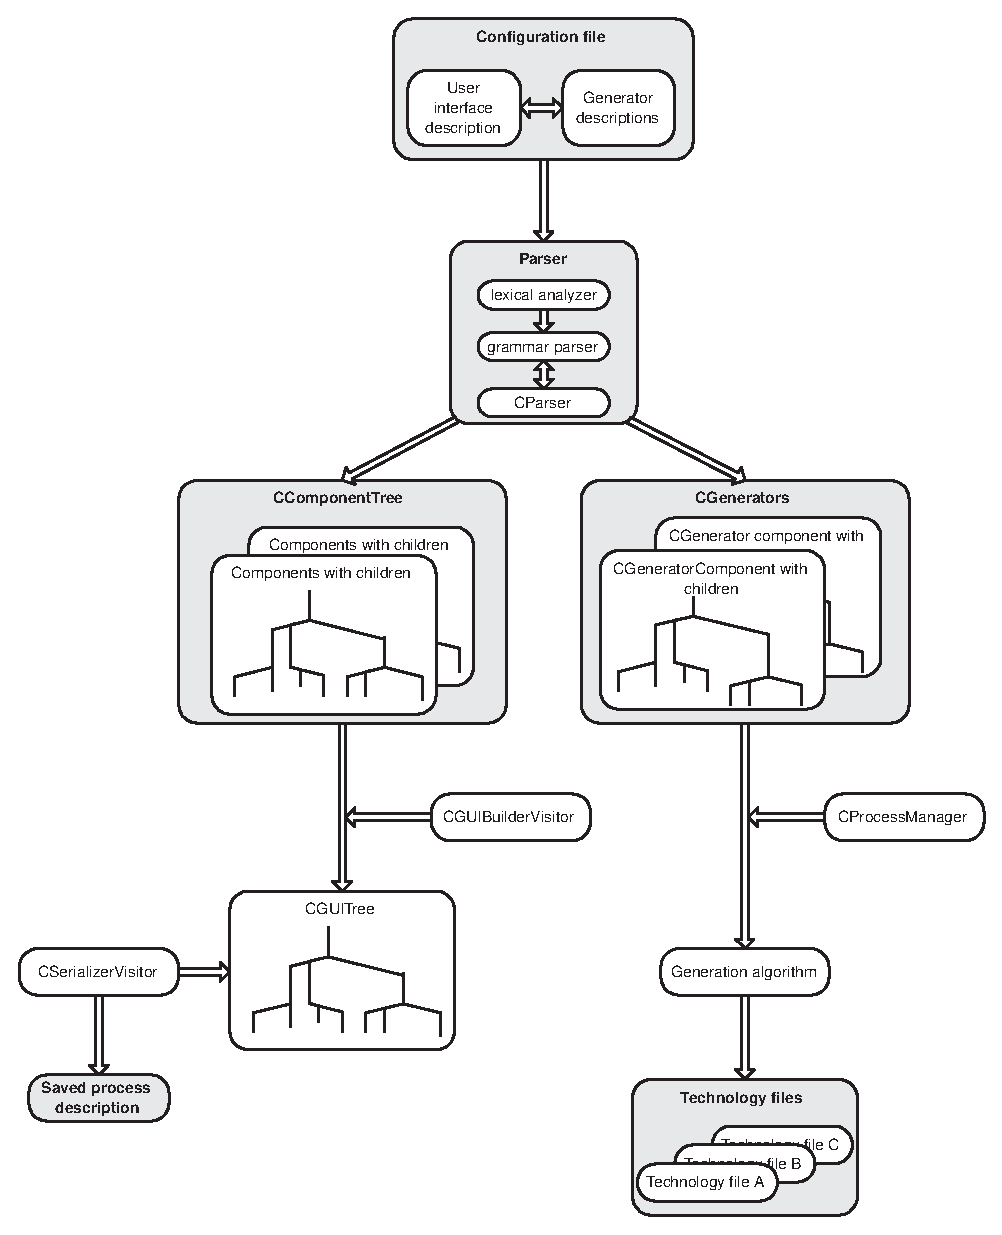
\includegraphics[height=10cm]{./figures/complete_overview.eps}
\caption{Complete architecture overview}
\label{fig:design:complete_overview}
\end{center} \end{figure}

\bigskip \noindent
Figure \ref{fig:design:complete_class} contains the class diagram as reverse
engineered by Rational Rose (a graphical design tool). Associations due to
connected signals and slots are not shown here, since Rational Rose cannot
handle these special Qt constructs.

The central role of the \verb=CGUITree= and \verb=CComponent= tree class is
quite clear.

\begin{figure} \begin{center}
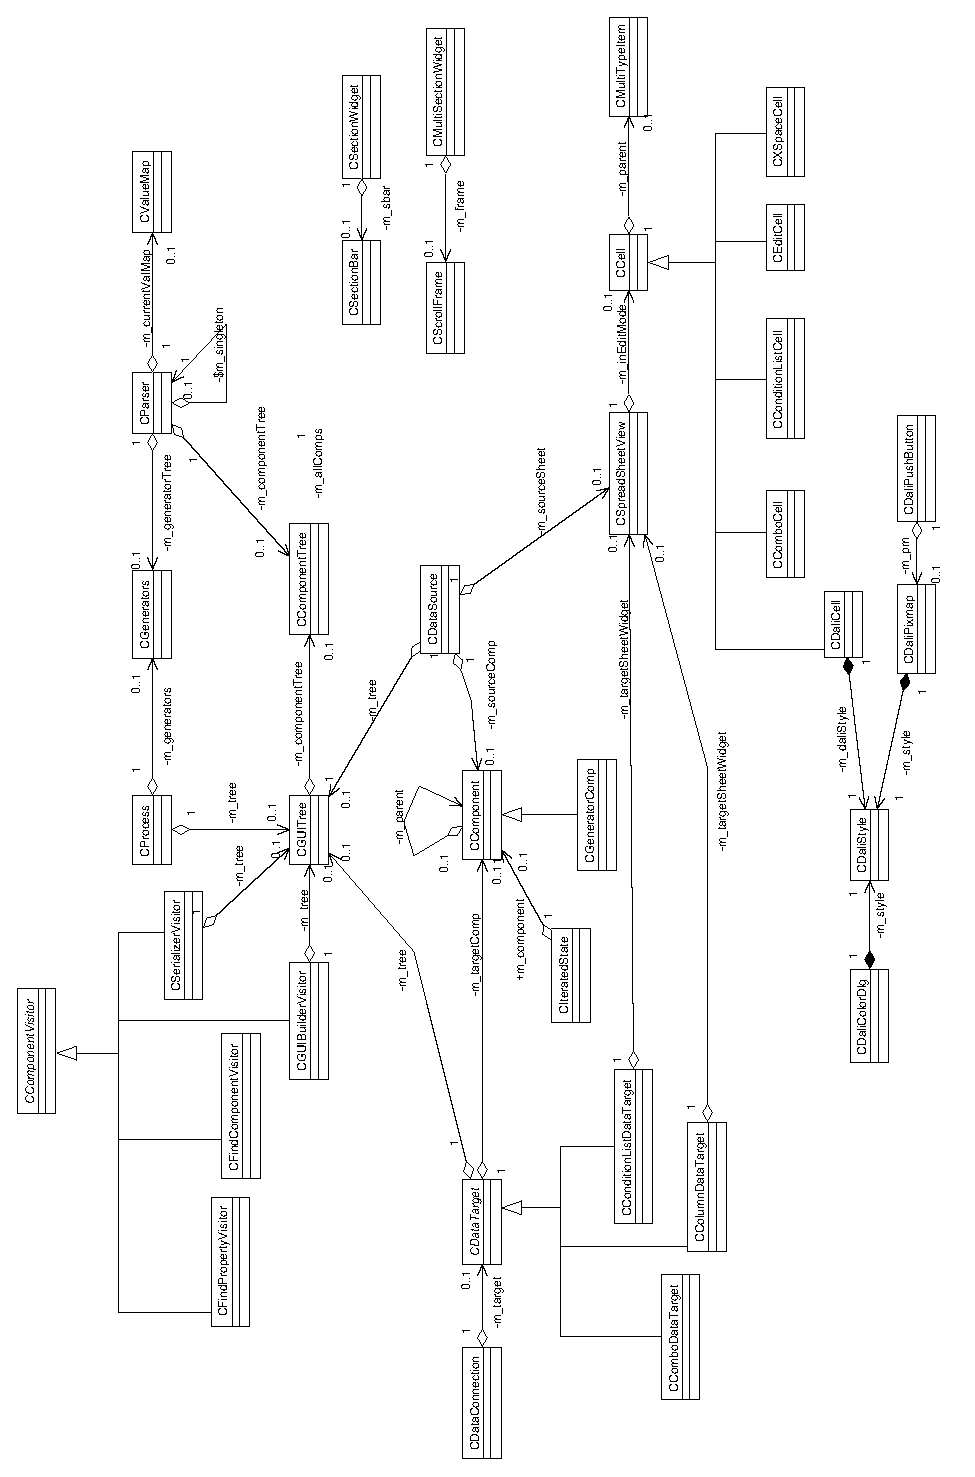
\includegraphics[width=12cm]{./figures/complete_class_diagram.eps}
\caption{Class diagram as reverse engineered by Rational Rose 2000}
\label{fig:design:complete_class}
\end{center} \end{figure}
